\section{Networking}
\label{sec:networking}
The engine will support multiplayer.
As the customer wants the engine to follow the Unity engine API, the multiplayer system wil follow the multiplayer package of unity \textbf{Netcode}.

\subsection{Network library}
Multiple libraries have been considered, for example ENet, RakNet or Boost.
The uses library is SLikeNet. This library is a continuation of RakNet, which is a well known and well documented library.
The library is also easy to use and has a lot of features that are useful for the engine.

\subsection{Class diagram}

\begin{figure}[H]
    \centering
    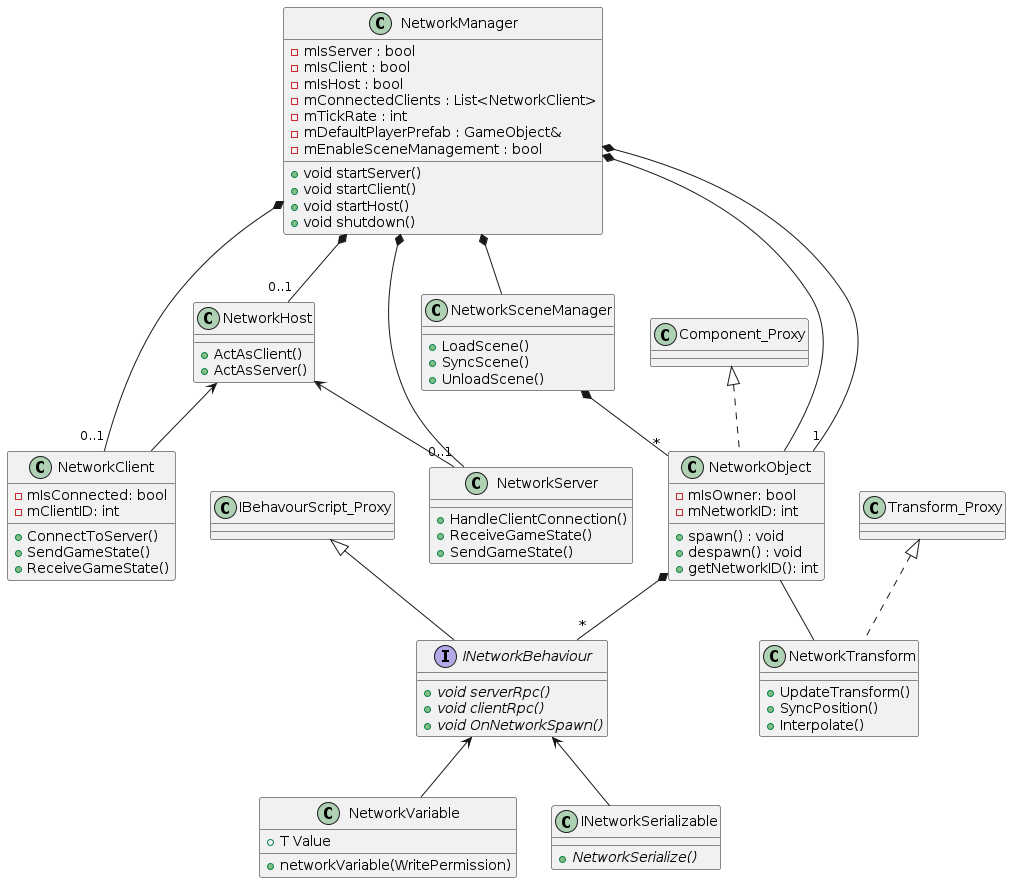
\includegraphics[width=\textwidth]{networkingClassDiagram.png}
    \caption{class diagram of the networking system}
    \label{fig:networkingClassDiagram}
\end{figure}
In \autoref{fig:networkingClassDiagram} the proxy classes are classes that are defined in a different class diagram.

A central manager named NetworkManager is used to manage the networking features.
An application can either be a server, a client or both and is then named a host.
To send information over the network a NetworkObject is used.
This object inherits Component class and can be added to a GameObject to define that this object can be sent over the network.
NetworkBehaviour inherits the behaviour class and can be used to send specific information over the network.
The NetworkTransform is used as a standard implemenation of sending the transform information over the network.
If a game programmer wants more control of what information is send when it should send this information with the NetworkBehaviour.

To send information over the network a NetworkVariable must be used.
This is a template class that defines information and how that information can be serialized.
